\documentclass[11pt, a4paper]{jsarticle}
\usepackage[dvipdfmx]{graphicx}
\begin{document}
\noindent
operating system 問題2-1\\
氏名:205759A 比嘉和樹\\
提出日:2021/1/3

\section{実験前の考察}
ファイルシステムはOSとは独立しているが、現在多くのOSがサポートしている。
これはメモリを分割してファイルとして割り当て、ディレクトリの構造の概念をメモリに持たせるものである。
goのプログラムはpackage osを使用することでOSと連携し、ファイルへの書き込みを実現する。
package osのFile構造体にはWrite関数が設定されており、これはbyte型の引数に含まれる文字列をFile構造体で指定したファイルに書き込む。
このとき引数とするbyte型で指定したデータを一気にOSに渡し、ファイルI/O処理の回数を減らすのがgolangのファイル書き込みにおけるバッファリングの手法である。
このことから、バッファのサイズを大きくするごとに、ファイルI/Oの回数はより減ることになり、処理時間はその分だけ短くなることと、ファイルサイズが大きくなるごとにその影響は顕著となることが予想できる。

今回の実験では、$2^2$~$2^{12}$のバッファサイズでデータファイルの大きさが5MBになるように書き込みを行い、その処理時間を測る手順を10回繰り返した。
その後、各バッファサイズについて処理時間の平均値を求め、1MBを書き込む秒数として処理速度を求めた。
図\ref{1}は、そのグラフである。

\begin{figure}[htbp]
	\centering
	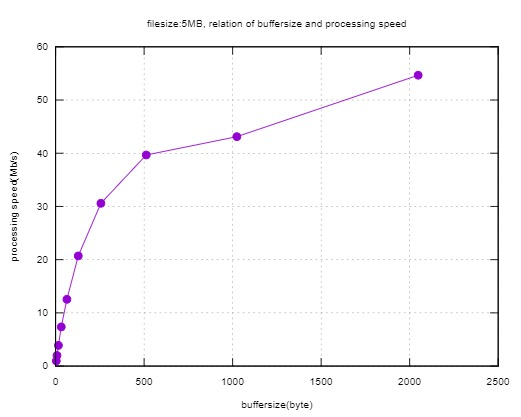
\includegraphics[width=100mm]{../out/out.jpg}
	\caption{バッファサイズと処理速度の関連}
	\label{1}
\end{figure}
\end{document}